\documentclass{standalone}
\usepackage{tikz}
\usetikzlibrary{patterns, positioning}

\begin{document}
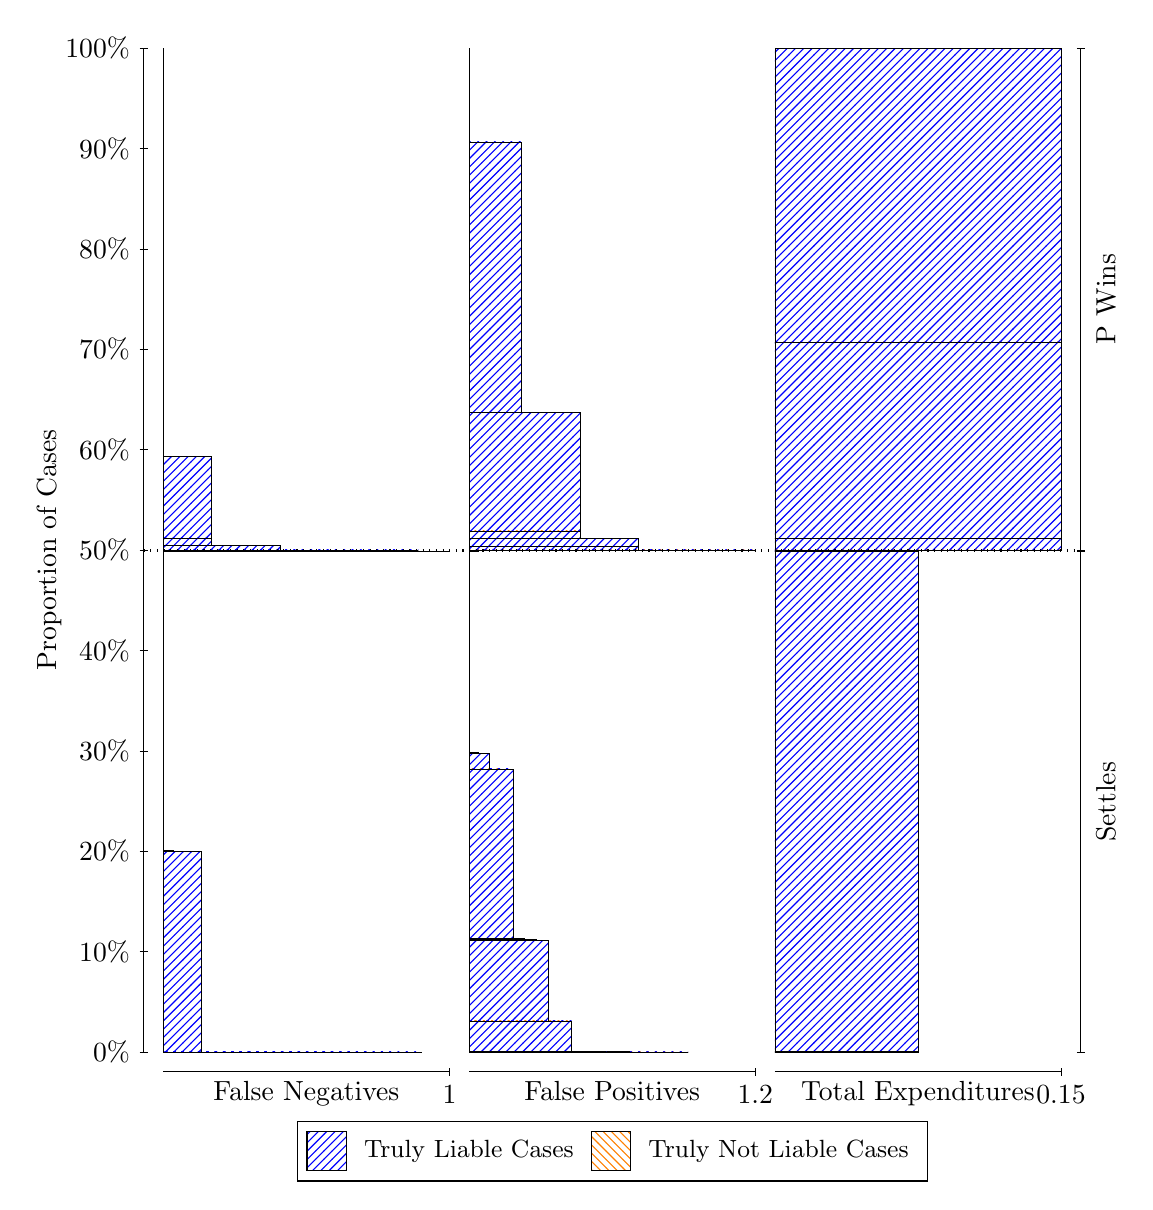
\begin{tikzpicture}
\draw[black, very thin] (1.5,1.75) -- (1.5,14.5);
\node[rotate=90, anchor=center] at (0.3, 8.125) {Proportion of Cases};
\draw[black, very thin] (1.45,1.75) -- (1.55,1.75);
\node[anchor=east] at (1.45, 1.75) {0\%};
\draw[black, very thin] (1.45,3.025) -- (1.55,3.025);
\node[anchor=east] at (1.45, 3.025) {10\%};
\draw[black, very thin] (1.45,4.3) -- (1.55,4.3);
\node[anchor=east] at (1.45, 4.3) {20\%};
\draw[black, very thin] (1.45,5.575) -- (1.55,5.575);
\node[anchor=east] at (1.45, 5.575) {30\%};
\draw[black, very thin] (1.45,6.85) -- (1.55,6.85);
\node[anchor=east] at (1.45, 6.85) {40\%};
\draw[black, very thin] (1.45,8.125) -- (1.55,8.125);
\node[anchor=east] at (1.45, 8.125) {50\%};
\draw[black, very thin] (1.45,9.4) -- (1.55,9.4);
\node[anchor=east] at (1.45, 9.4) {60\%};
\draw[black, very thin] (1.45,10.675) -- (1.55,10.675);
\node[anchor=east] at (1.45, 10.675) {70\%};
\draw[black, very thin] (1.45,11.95) -- (1.55,11.95);
\node[anchor=east] at (1.45, 11.95) {80\%};
\draw[black, very thin] (1.45,13.225) -- (1.55,13.225);
\node[anchor=east] at (1.45, 13.225) {90\%};
\draw[black, very thin] (1.45,14.5) -- (1.55,14.5);
\node[anchor=east] at (1.45, 14.5) {100\%};

\draw[black, very thin] (13.4,1.75) -- (13.4,14.5);
\draw[black, very thin] (13.35,1.75) -- (13.45,1.75);
\node[anchor=west] at (13.35, 1.75) {};
\draw[black, very thin] (13.35,8.1029) -- (13.45,8.1029);
\node[anchor=west] at (13.35, 8.1029) {};
\draw[black, very thin] (13.35,8.1256) -- (13.45,8.1256);
\node[anchor=west] at (13.35, 8.1256) {};
\draw[black, very thin] (13.35,14.5) -- (13.45,14.5);
\node[anchor=west] at (13.35, 14.5) {};

\draw[black, very thin, pattern color=blue, pattern=north east lines] (1.75,1.75) rectangle (5.0331,1.75);
\draw[black, very thin, pattern color=blue, pattern=north east lines] (1.75,1.75) rectangle (4.6829,1.75);
\draw[black, very thin, pattern color=blue, pattern=north east lines] (1.75,1.75) rectangle (4.3327,1.75);
\draw[black, very thin, pattern color=blue, pattern=north east lines] (1.75,1.75) rectangle (4.1576,1.75);
\draw[black, very thin, pattern color=blue, pattern=north east lines] (1.75,1.75) rectangle (3.9825,1.75);
\draw[black, very thin, pattern color=blue, pattern=north east lines] (1.75,1.75) rectangle (3.8074,1.75);
\draw[black, very thin, pattern color=blue, pattern=north east lines] (1.75,1.75) rectangle (3.6323,1.75);
\draw[black, very thin, pattern color=blue, pattern=north east lines] (1.75,1.75) rectangle (3.4572,1.75);
\draw[black, very thin, pattern color=blue, pattern=north east lines] (1.75,1.75) rectangle (3.2821,1.75);
\draw[black, very thin, pattern color=blue, pattern=north east lines] (1.75,1.75) rectangle (3.107,1.75);
\draw[black, very thin, pattern color=blue, pattern=north east lines] (1.75,1.75) rectangle (3.107,1.75);
\draw[black, very thin, pattern color=blue, pattern=north east lines] (1.75,1.75) rectangle (2.9319,1.75);
\draw[black, very thin, pattern color=blue, pattern=north east lines] (1.75,1.75) rectangle (2.7568,1.75);
\draw[black, very thin, pattern color=blue, pattern=north east lines] (1.75,1.75) rectangle (2.5817,1.7514);
\draw[black, very thin, pattern color=blue, pattern=north east lines] (1.75,1.7514) rectangle (2.5817,1.7514);
\draw[black, very thin, pattern color=blue, pattern=north east lines] (1.75,1.7514) rectangle (2.4066,1.7516);
\draw[black, very thin, pattern color=blue, pattern=north east lines] (1.75,1.7516) rectangle (2.2315,1.7516);
\draw[black, very thin, pattern color=blue, pattern=north east lines] (1.75,1.7516) rectangle (2.2315,4.2978);
\draw[black, very thin, pattern color=blue, pattern=north east lines] (1.75,4.2978) rectangle (2.0564,4.2984);
\draw[black, very thin, pattern color=blue, pattern=north east lines] (1.75,4.2984) rectangle (2.0564,4.2988);
\draw[black, very thin, pattern color=blue, pattern=north east lines] (1.75,4.2988) rectangle (1.8813,4.3093);
\draw[black, very thin, pattern color=orange, pattern=north west lines] (1.75,4.3093) rectangle (1.75,4.3093);
\draw[black, very thin, pattern color=blue, pattern=north east lines] (1.75,4.3093) rectangle (1.75,8.1029);
\draw[black, very thin, pattern color=blue, pattern=north east lines] (1.75,8.1029) rectangle (5.3833,8.1029);
\draw[black, very thin, pattern color=blue, pattern=north east lines] (1.75,8.1029) rectangle (4.5078,8.1029);
\draw[black, very thin, pattern color=blue, pattern=north east lines] (1.75,8.1029) rectangle (3.6323,8.1029);
\draw[black, very thin, pattern color=blue, pattern=north east lines] (1.75,8.1029) rectangle (2.7568,8.1064);
\draw[black, very thin, pattern color=blue, pattern=north east lines] (1.75,8.1064) rectangle (1.8813,8.1256);
\draw[black, very thin, pattern color=orange, pattern=north west lines] (1.75,8.1256) rectangle (1.75,8.1256);
\draw[black, very thin, pattern color=blue, pattern=north east lines] (1.75,8.1256) rectangle (4.9894,8.1256);
\draw[black, very thin, pattern color=blue, pattern=north east lines] (1.75,8.1256) rectangle (4.1139,8.1258);
\draw[black, very thin, pattern color=blue, pattern=north east lines] (1.75,8.1258) rectangle (3.2384,8.1259);
\draw[black, very thin, pattern color=blue, pattern=north east lines] (1.75,8.1259) rectangle (3.2384,8.1828);
\draw[black, very thin, pattern color=blue, pattern=north east lines] (1.75,8.1828) rectangle (2.3629,8.2793);
\draw[black, very thin, pattern color=blue, pattern=north east lines] (1.75,8.2793) rectangle (2.3629,9.3165);
\draw[black, very thin, pattern color=orange, pattern=north west lines] (1.75,9.3165) rectangle (1.75,9.3165);
\draw[black, very thin, pattern color=blue, pattern=north east lines] (1.75,9.3165) rectangle (1.75,14.5);
\draw[black, very thin, pattern color=orange, pattern=north west lines] (5.6333,1.75) rectangle (8.4139,1.75);
\draw[black, very thin, pattern color=blue, pattern=north east lines] (5.6333,1.75) rectangle (8.4139,1.75);
\draw[black, very thin, pattern color=orange, pattern=north west lines] (5.6333,1.75) rectangle (8.1173,1.75);
\draw[black, very thin, pattern color=blue, pattern=north east lines] (5.6333,1.75) rectangle (8.1173,1.75);
\draw[black, very thin, pattern color=orange, pattern=north west lines] (5.6333,1.75) rectangle (7.8207,1.75);
\draw[black, very thin, pattern color=blue, pattern=north east lines] (5.6333,1.75) rectangle (7.8207,1.75);
\draw[black, very thin, pattern color=blue, pattern=north east lines] (5.6333,1.75) rectangle (7.6724,1.7526);
\draw[black, very thin, pattern color=orange, pattern=north west lines] (5.6333,1.7526) rectangle (7.5241,1.7526);
\draw[black, very thin, pattern color=blue, pattern=north east lines] (5.6333,1.7526) rectangle (7.5241,1.7526);
\draw[black, very thin, pattern color=blue, pattern=north east lines] (5.6333,1.7526) rectangle (7.3759,1.7526);
\draw[black, very thin, pattern color=orange, pattern=north west lines] (5.6333,1.7526) rectangle (7.2276,1.7526);
\draw[black, very thin, pattern color=blue, pattern=north east lines] (5.6333,1.7526) rectangle (7.2276,1.7526);
\draw[black, very thin, pattern color=blue, pattern=north east lines] (5.6333,1.7526) rectangle (7.0793,1.7531);
\draw[black, very thin, pattern color=orange, pattern=north west lines] (5.6333,1.7531) rectangle (6.931,1.7531);
\draw[black, very thin, pattern color=blue, pattern=north east lines] (5.6333,1.7531) rectangle (6.931,2.1454);
\draw[black, very thin, pattern color=orange, pattern=north west lines] (5.6333,2.1454) rectangle (6.931,2.1454);
\draw[black, very thin, pattern color=blue, pattern=north east lines] (5.6333,2.1454) rectangle (6.931,2.1454);
\draw[black, very thin, pattern color=blue, pattern=north east lines] (5.6333,2.1454) rectangle (6.7827,2.1458);
\draw[black, very thin, pattern color=blue, pattern=north east lines] (5.6333,2.1458) rectangle (6.6344,2.1458);
\draw[black, very thin, pattern color=orange, pattern=north west lines] (5.6333,2.1458) rectangle (6.6344,2.1458);
\draw[black, very thin, pattern color=blue, pattern=north east lines] (5.6333,2.1458) rectangle (6.6344,3.166);
\draw[black, very thin, pattern color=blue, pattern=north east lines] (5.6333,3.166) rectangle (6.4861,3.1768);
\draw[black, very thin, pattern color=orange, pattern=north west lines] (5.6333,3.1768) rectangle (6.3378,3.1768);
\draw[black, very thin, pattern color=blue, pattern=north east lines] (5.6333,3.1768) rectangle (6.3378,3.1793);
\draw[black, very thin, pattern color=blue, pattern=north east lines] (5.6333,3.1793) rectangle (6.3378,3.1917);
\draw[black, very thin, pattern color=blue, pattern=north east lines] (5.6333,3.1917) rectangle (6.1895,5.3449);
\draw[black, very thin, pattern color=blue, pattern=north east lines] (5.6333,5.3449) rectangle (6.1895,5.3449);
\draw[black, very thin, pattern color=orange, pattern=north west lines] (5.6333,5.3449) rectangle (6.0412,5.3449);
\draw[black, very thin, pattern color=blue, pattern=north east lines] (5.6333,5.3449) rectangle (6.0412,5.346);
\draw[black, very thin, pattern color=blue, pattern=north east lines] (5.6333,5.346) rectangle (6.0412,5.3464);
\draw[black, very thin, pattern color=blue, pattern=north east lines] (5.6333,5.3464) rectangle (5.8929,5.3464);
\draw[black, very thin, pattern color=blue, pattern=north east lines] (5.6333,5.3464) rectangle (5.8929,5.5436);
\draw[black, very thin, pattern color=blue, pattern=north east lines] (5.6333,5.5436) rectangle (5.7446,5.5541);
\draw[black, very thin, pattern color=blue, pattern=north east lines] (5.6333,5.5541) rectangle (5.6333,8.1029);
\draw[black, very thin, pattern color=orange, pattern=north west lines] (5.6333,8.1029) rectangle (5.7446,8.1029);
\draw[black, very thin, pattern color=blue, pattern=north east lines] (5.6333,8.1029) rectangle (5.7446,8.122);
\draw[black, very thin, pattern color=blue, pattern=north east lines] (5.6333,8.122) rectangle (5.6333,8.1256);
\draw[black, very thin, pattern color=orange, pattern=north west lines] (5.6333,8.1256) rectangle (9.2667,8.1256);
\draw[black, very thin, pattern color=blue, pattern=north east lines] (5.6333,8.1256) rectangle (9.2667,8.1256);
\draw[black, very thin, pattern color=blue, pattern=north east lines] (5.6333,8.1256) rectangle (8.5252,8.1266);
\draw[black, very thin, pattern color=orange, pattern=north west lines] (5.6333,8.1266) rectangle (8.5252,8.1266);
\draw[black, very thin, pattern color=blue, pattern=north east lines] (5.6333,8.1266) rectangle (8.5252,8.1275);
\draw[black, very thin, pattern color=blue, pattern=north east lines] (5.6333,8.1275) rectangle (7.7837,8.1751);
\draw[black, very thin, pattern color=orange, pattern=north west lines] (5.6333,8.1751) rectangle (7.7837,8.1751);
\draw[black, very thin, pattern color=blue, pattern=north east lines] (5.6333,8.1751) rectangle (7.7837,8.2732);
\draw[black, very thin, pattern color=blue, pattern=north east lines] (5.6333,8.2732) rectangle (7.0422,8.3685);
\draw[black, very thin, pattern color=orange, pattern=north west lines] (5.6333,8.3685) rectangle (7.0422,8.3685);
\draw[black, very thin, pattern color=blue, pattern=north east lines] (5.6333,8.3685) rectangle (7.0422,9.8687);
\draw[black, very thin, pattern color=blue, pattern=north east lines] (5.6333,9.8687) rectangle (6.3007,9.8714);
\draw[black, very thin, pattern color=orange, pattern=north west lines] (5.6333,9.8714) rectangle (6.3007,9.8714);
\draw[black, very thin, pattern color=blue, pattern=north east lines] (5.6333,9.8714) rectangle (6.3007,13.309);
\draw[black, very thin, pattern color=blue, pattern=north east lines] (5.6333,13.309) rectangle (5.6333,14.5);
\draw[black, very thin, pattern color=orange, pattern=north west lines] (9.5167,1.75) rectangle (11.333,1.75);
\draw[black, very thin, pattern color=blue, pattern=north east lines] (9.5167,1.75) rectangle (11.333,1.7543);
\draw[black, very thin, pattern color=orange, pattern=north west lines] (9.5167,1.7543) rectangle (11.333,1.7543);
\draw[black, very thin, pattern color=blue, pattern=north east lines] (9.5167,1.7543) rectangle (11.333,8.1029);
\draw[black, very thin, pattern color=orange, pattern=north west lines] (9.5167,8.1029) rectangle (11.333,8.1029);
\draw[black, very thin, pattern color=blue, pattern=north east lines] (9.5167,8.1029) rectangle (11.333,8.1256);
\draw[black, very thin, pattern color=orange, pattern=north west lines] (9.5167,8.1256) rectangle (13.15,8.1256);
\draw[black, very thin, pattern color=blue, pattern=north east lines] (9.5167,8.1256) rectangle (13.15,8.2722);
\draw[black, very thin, pattern color=orange, pattern=north west lines] (9.5167,8.2722) rectangle (13.15,8.2722);
\draw[black, very thin, pattern color=blue, pattern=north east lines] (9.5167,8.2722) rectangle (13.15,10.767);
\draw[black, very thin, pattern color=orange, pattern=north west lines] (9.5167,10.767) rectangle (13.15,10.767);
\draw[black, very thin, pattern color=blue, pattern=north east lines] (9.5167,10.767) rectangle (13.15,14.5);
\draw[black, dotted] (1.5,8.1029) -- (13.4,8.1029);
\draw[black, dotted] (1.5,8.1256) -- (13.4,8.1256);
\draw[black, very thin] (1.75,1.5) -- (5.3833,1.5);
\node[anchor=north] at (3.5667, 1.5) {False Negatives};
\draw[black, very thin] (5.3833,1.45) -- (5.3833,1.55);
\node[anchor=north] at (5.3833, 1.45) {1};

\draw[black, very thin] (5.6333,1.5) -- (9.2667,1.5);
\node[anchor=north] at (7.45, 1.5) {False Positives};
\draw[black, very thin] (9.2667,1.45) -- (9.2667,1.55);
\node[anchor=north] at (9.2667, 1.45) {1.2};

\draw[black, very thin] (9.5167,1.5) -- (13.15,1.5);
\node[anchor=north] at (11.333, 1.5) {Total Expenditures};
\draw[black, very thin] (13.15,1.45) -- (13.15,1.55);
\node[anchor=north] at (13.15, 1.45) {0.15};

\node[black, centered, rotate=90] at (13.72, 4.9264) {Settles};

\node[black, centered, rotate=90] at (13.72, 11.313) {P Wins};

\draw (7.449999999999999,1.5) node[draw=none] (baseCoordinate) {};
\begin{scope}[align=center]
        \matrix[scale=0.5, draw=black, below=0.5cm of baseCoordinate, nodes={draw}, column sep=0.1cm]{
            \node[rectangle, draw, minimum width=0.5cm, minimum height=0.5cm, pattern=north east lines, pattern color=blue] {}; &
            \node[draw=none, font=\small] (B) {Truly Liable Cases}; &
            \node[rectangle, draw, minimum width=0.5cm, minimum height=0.5cm, pattern=north west lines, pattern color=orange] {}; &
            \node[draw=none, font=\small] (B) {Truly Not Liable Cases}; \\
            };
\end{scope}

\end{tikzpicture}
\end{document}